\chapter{Introduction} \label{chap:introduction}
Your intro... Thesis ref example: \cite{bulin:2016}, Misc ref example: \cite{smidl:pc}, Article ref example: \cite{mcculloch:neuron}, Online webpage ref example: \cite{online:xor_solution}

\section{State of the Art} \label{sec:state_of_the_art}

% /** General

The most famous intelligent personal assistants include Alexa, Siri, Google Assistant. These virtual assistants work on a very similar principle as follows. The assistant constantly listens to its surroundings to see if a wake-up word has been spoken. Assistant process this analysis of wake-up word on its hardware. After saying the wake-up word, the assistant starts recording a sound and analyzes simultaneously if no one is talking anymore. This recorded sound then assistant send to the appropriate servers for processing. The server handles the relevant device or service according to the processed user command and sends a synthesized audio response back to the assistant.

Siri's first assistant was created by Apple in 2010 and shortly followed by Cortana by Microsoft in 2013 and Alexa by Amazon in 2014. The growing power of computers and advancing cloud technology allows scientists and software engineers to train voice assistants more easily. Over time, voice assistants can respond to the user more naturally and give the user the feeling of talking to a person. 

In addition to these tasks, the user can connect the voice assistant to web services (see \cref{fig:voice_assistant_connecrtion_schema}) like Tasker, IFTTT and other features (often called "skills") developed by third-party developers. By these additions, the user adds a new palette of commands such as automating social media posts, ordering a usual drink from a local Starbucks or summoning an Uber or Lyft using connected account data.

\begin{figure}[H]
    \centering
    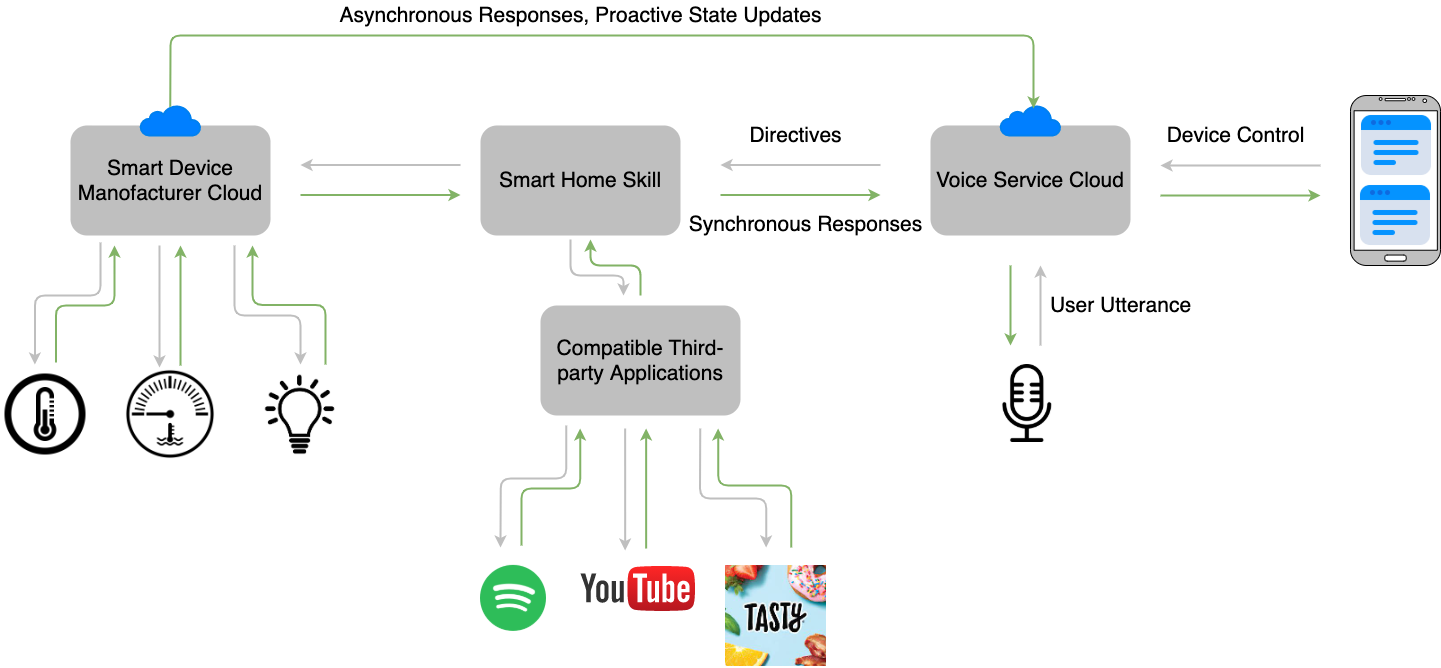
\includegraphics[width=\textwidth]{img/voice_assistant_to_server_connection.png}
    \caption{Connection schema of voice assistant service}
    \label{fig:voice_assistant_connecrtion_schema}
\end{figure}

Although each currently available voice assistant has unique features, they share some similarities and are able to perform the following basic tasks \citep{voice_assistants_general_hoy_2018}: 

\begin{itemize}
    \item send and read text messages, make phone calls, and send and read email messages; 
    \item answer basic informational queries (“What time is it? What’s the weather forecast? How many ounces are in a cup?”); 
    \item set timers, alarms, and calendar entries;
    \item set reminders, make lists, and do basic math calculations;
    \item control media playback from connected services such as Amazon, Google Play, iTunes, Pandora, Netflix, and Spotify; 
    \item control  Internet-of-Things-enabled  devices  such  as  thermostats,  lights, alarms, and locks; and 
    \item tell jokes and stories. 
\end{itemize}

\subsection{Comparison between Google Assistant, Siri, Alexa}

Because each company develop its voice assistant independently and protect its knowledge, these assistants are quite different despite their common ground. Figure \cref{fig:voice_assistant_comparison} determine the most capable assistant by asking 800 questions that consist of categories like \citep{voice_assistant_comparison_munster_2019}:

\begin{itemize}
    \item Local – Where is the nearest coffee shop?
    \item Commerce – Order me more paper towels.
    \item Navigation – How do I get to Uptown on the bus?
    \item Information – Who do the Twins play tonight?
    \item Command – Remind me to call Jerome at 2 pm today.
\end{itemize}

\begin{figure}[H]
    \centering
    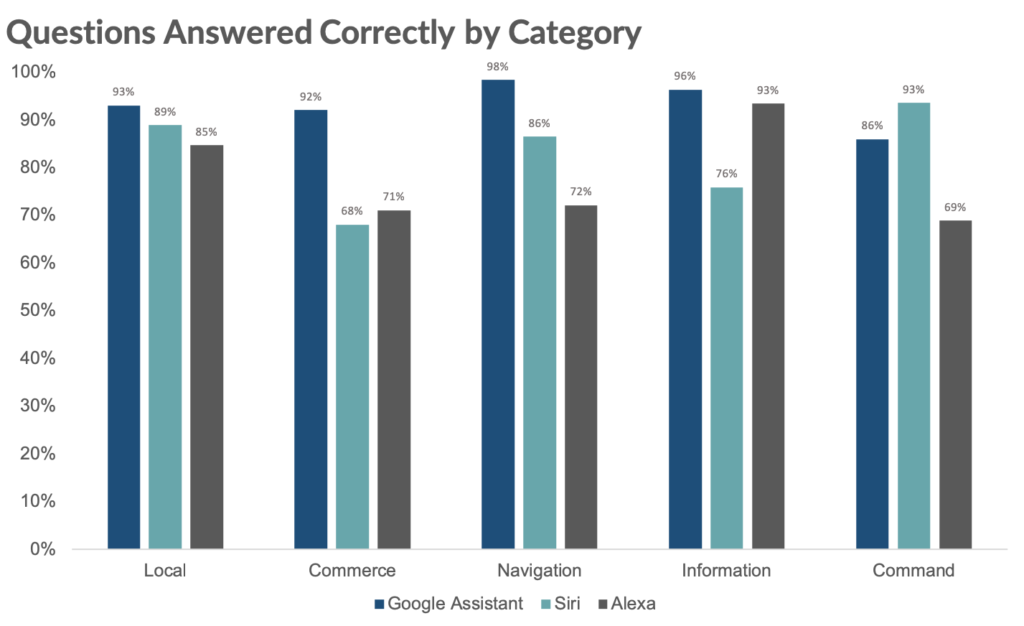
\includegraphics[width=\textwidth]{img/voice_assistant_comparison.png}
    \caption{Voice assistant comparison by types of questions}
    \label{fig:voice_assistant_comparison}
\end{figure}

Google Assistant has answered 93\% correctly and has understood all 800 questions correctly. Siri has been next, has answered 83\% correctly and has misunderstood only two questions. Alexa has answered 80\% correctly and has misunderstood only one. According to the data shown in \cref{fig:voice_assistant_comparison}, Google Assistant has better results overall but lacks in the command category. Amazon Alexa has excellent results only in the information category, where it climbs just below the results of Google Assistant. Siri is brilliant in the command category for such functions as a calling, sending SMS or playing music.

If several users occupy the room, each voice assistant has its way of handling this situation. For example, Amazon Alexa and Google Assistant create multiple voice profiles, which allows the user to train the assistant to recognize his voice specifically and therefore offer different data and use separate accounts for services. This is a very complex task, and no one can cope with it at the desired level.

% assistants comparison
% https://www.researchgate.net/publication/337407222_User_Experience_Comparison_of_Intelligent_Personal_Assistants_Alexa_Google_Assistant_Siri_and_Cortana

% https://www.researchgate.net/publication/329624889_Using_intelligent_personal_assistants_to_assist_the_elderlies_An_evaluation_of_Amazon_Alexa_Google_Assistant_Microsoft_Cortana_and_Apple_Siri



\section{Thesis Objectives} \label{sec:thesis_objectives}

% Až budeš psát thesis objectives, navrhuji držet se následujících bodů (souvisí s oficiálním zadáním práce):

% Hlavní cíl: navržení obecného komunikačního rozhraní pro hlasově ovládané moduly chytré domácnosti

% Dílčí cíle:
% 1/ otestování vybraných modulů pro využití v projektu
% 2/ fyzická realizace hardwarově závislých modulů
% 3/ řešení rozhraní mezi uživatelem a moduly (backend)
% 4/ přidání hlasové interakce
% 5/ dle časů a možností obohacení o další moduly


% Učeš to podle svého mínění, ale držel bych podobnou kostru.

\section{Thesis Outline} \label{sec:thesis_outline}
